% !TEX encoding = UTF-8
% !TEX TS-program = pdflatex
% !TEX root = ../elsarticle-template-num.tex
% !TEX spellcheck = en-EN

%************************************************
\section{Method}
\label{sec:method}
%************************************************
%\section{Method}
%\label{sec:method}
%************************************************

%%\lipsum[1]
%%\begin{equation}
\label{eq:emc}
e = mc^2
\end{equation}


\begin{figure}[!htb] 
\centering 
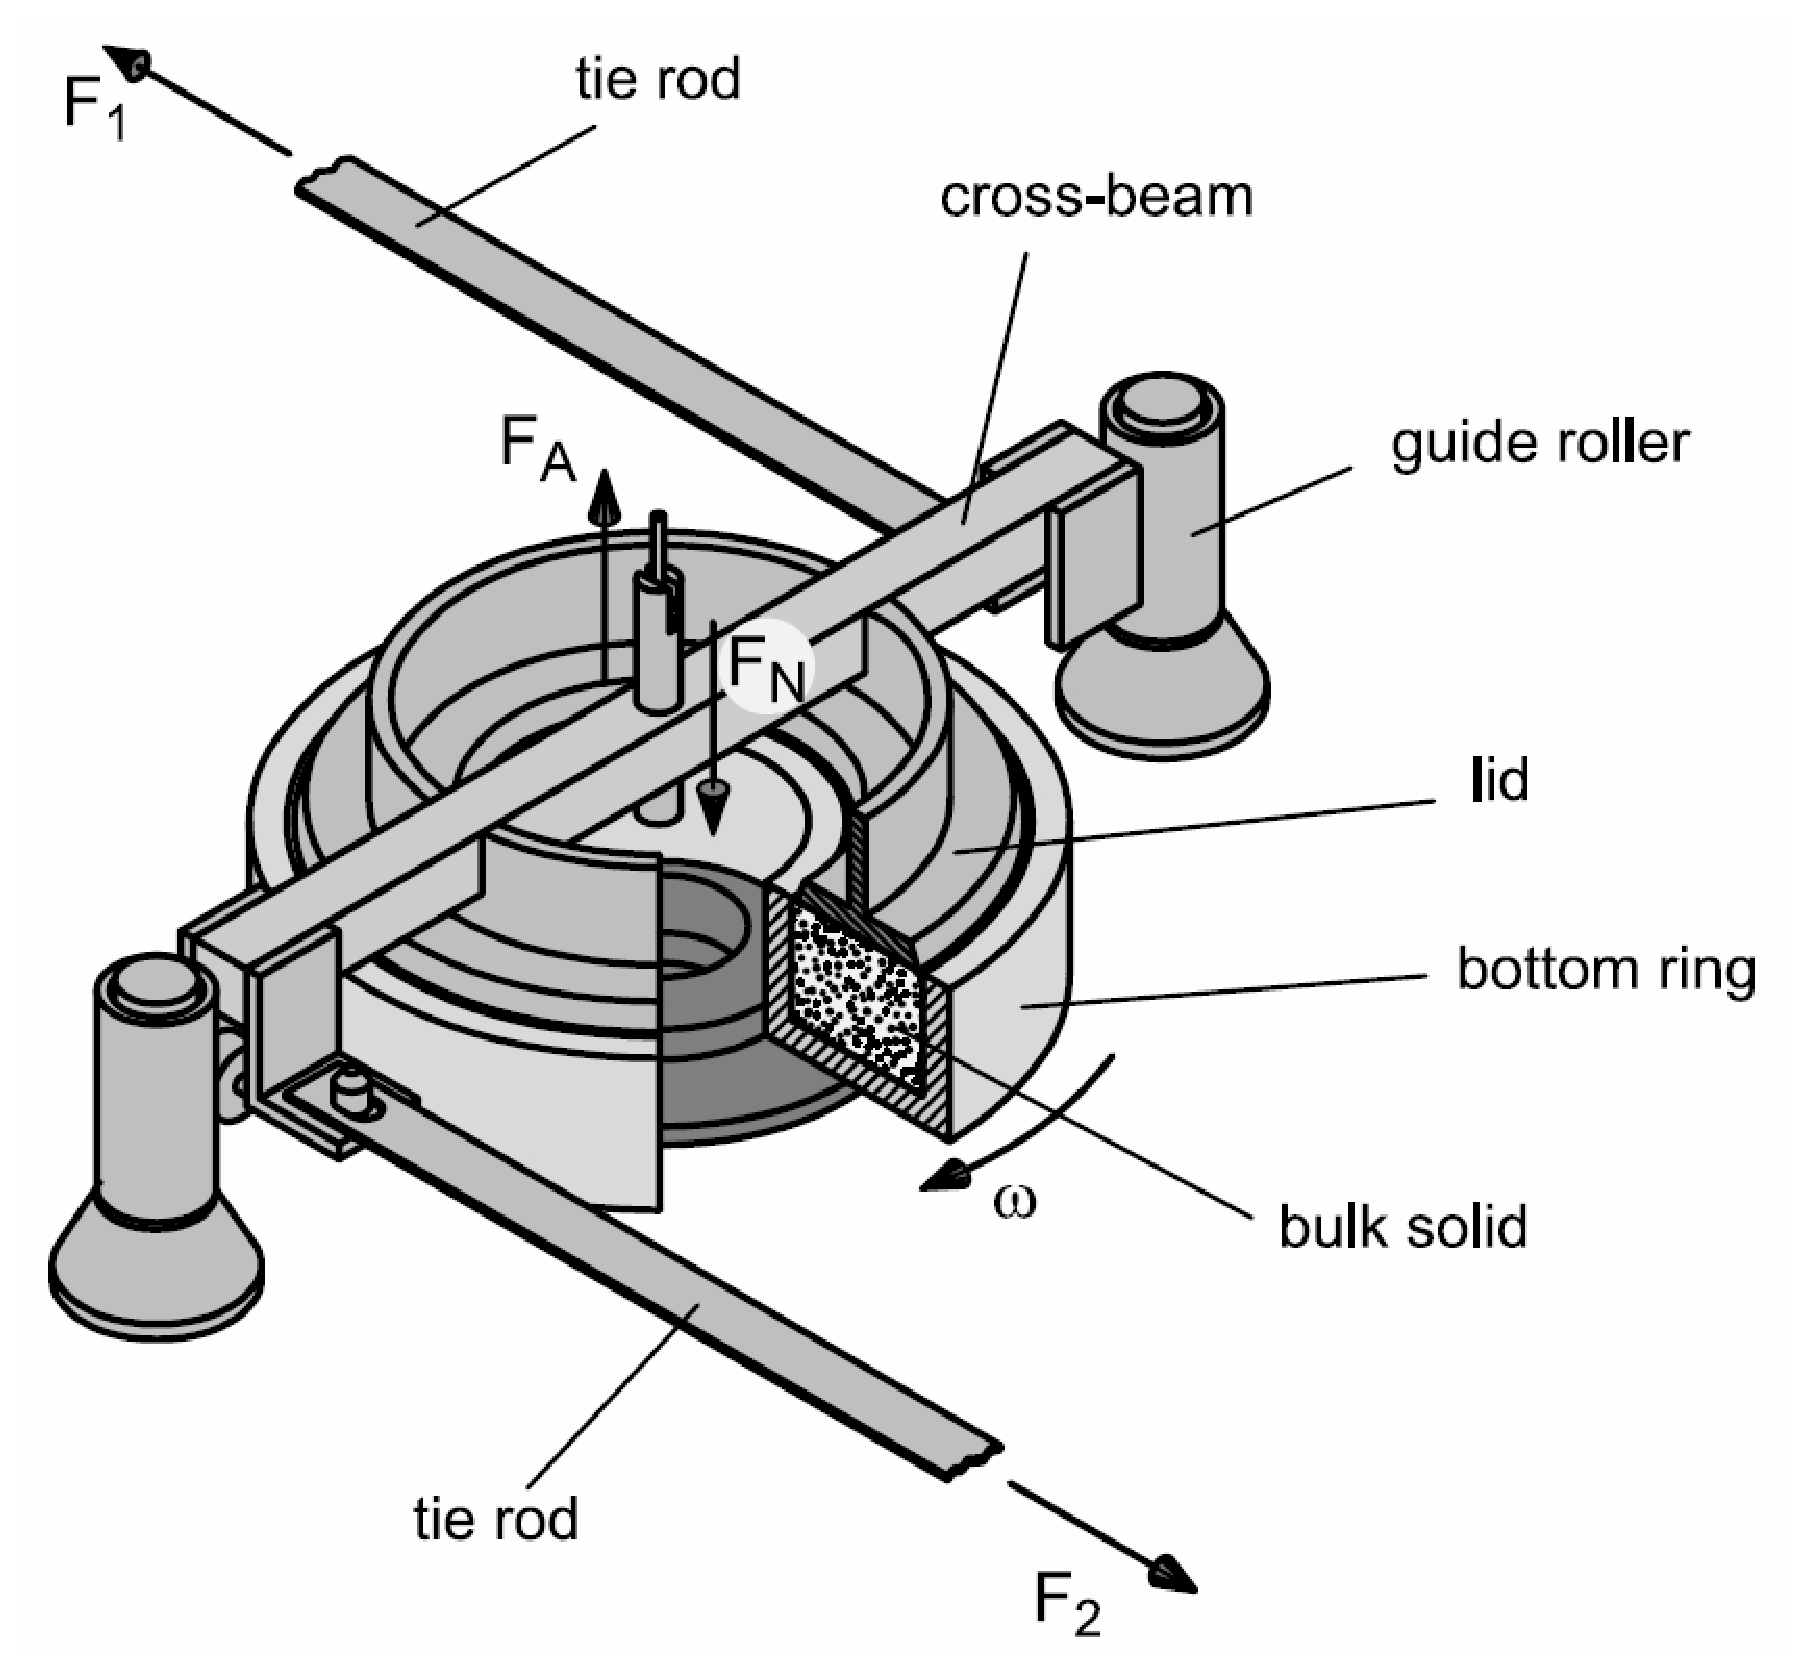
\includegraphics[width=.8\textwidth]{images/original/01srsct} 
\caption[Schulze ring shear cell tester]{Schulze ring shear cell tester
experimental layout, Schulze \cite{RefWorks:118}}
\label{fig:01srsct} 
\end{figure}


% \begin{figure}[htp]
%     \centering
%     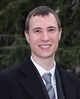
\includegraphics[width=.2\textwidth]{images/vitae/lbenvenuti}
%     \caption{OpenMP, MPI, MPI/OpenMP Hybrid runs of Box in a box testcase on 32
%     cores. The OpenMP-only run suffers from limited memory bandwidth in
%     memory-bound algorithms inside of the Modify section of the code. MPI-only has
%     low averaged runtimes for each section, but a very large Other timing, which
%     hints for a large amount of load-imbalance. Hybrid timings are a bit worse
%     on average, but because of better balancing, processes have lower wait times
%     inside of Other timing.}
% 	\label{fig:boxInBoxComparison}

aa
aaaaaa
%\input{images/texCaller/regressionTest}

\subsection{Discrete element method}
\label{subsec:dem}
The $DEM$ is based on a relatively elementary idea. For each particle i inside
the domain it follows the course and calculate the force of that exerts on particle j
by integrating Newton' second law:
\begin{equation}
m \ddot{x}_{ij} + c \dot{x}_{ij} + k x_{ij} =  F_{ij} .
\label{equ:newtonlaw}
\end{equation}

and the position and orientation equations.
Further details on the method can be found in \cite{RefWorks:133}.


Further details on the method can be found in \cite{RefWorks:133}.

The coefficient of sliding friction for coarse round particles is a critical
parameter describing inter-particle friction in medium to dense granular flows simulations.
It is proportional to the torque counteracting the rotation of the particle and defined as (Eq. \ref{equ:mur}):
\begin{equation}
 \mu_r =  \tan(\iota) .
\label{equ:mur}
\end{equation}


Furthermore, we used Hertz' Law for the particle-particle and particle-wall interactions.

\begin{equation}
 F_{ij} = 
\begin{cases}
F_{n,ij} + F_{t,ij} = \left( k_n \delta_{n,ij} + \gamma_n v_{n,ij} \right) + \left( k_t \delta_{t,ij} + \gamma_t v_{t,ij} \right) & \text{if } r < d ,\\
0    & \text{if } r > d ,\\
\end{cases}
 \label{eq:forceij}
\end{equation}


\subsection{Artificial Neural Networks}
\label{subsec:ann}
\lipsum[1]
\begin{equation}
\begin{aligned}
M_r &= M_r^k ,\\
M_{r,ti+\Delta ti}^k &= M_{r,ti}^k - k_r \Delta \theta_r ,\\
\lvert{M_{r,ti+\Delta ti}^k}\rvert & \leq M_r^m = \mu_r R_{eq} F_n .\\
\end{aligned}
 \label{eq:mrtm}
\end{equation}


\subsection{Experimental setup}
\label{subsec:experimentalsetup}
\lipsum[1]
\begin{equation}
\begin{aligned}
 \frac{1}{E_{eq}} & = \frac{1-\nu_i^2}{E_i} + \frac{1-\nu_j^2}{E_j} ,\\
 \frac{1}{G_{eq}} & = \frac{2(2+\nu_i)(1-\nu_i)}{E_i} + \frac{2(2+\nu_j)(1-\nu_j)}{E_j} ,\\
 \frac{1}{R_{eq}} &= \frac{1}{R_i} + \frac{1}{R_j} ,\\
 \frac{1}{m_{eq}} &= \frac{1}{m_i} + \frac{1}{m_j} ,\\
 \beta & = \frac{\ln(e)}{\sqrt{ln^2(e)+\pi^2}} ,\\
 S_n & = 2 E_{eq} \sqrt{R_{eq} \delta_n} ,\\
 S_t & = 8 G_{eq} \sqrt{R_{eq} \delta_n} ,\\
 k_r & = k_t R_{eq}^2 .\\
\end{aligned}
\label{eq:equivProp2}
\end{equation}



